\newpage

\section{Dynamo: Amazon's Highly Available Key-Value Store}

It's 2007 and Amazon's global e-commerce platform must remain ``always-on'' despite continual component failures, outages cost revenue and customer trust. To achieve this, Dynamo sacrifices strict consistency for low-latency availability:

\begin{Def}[Design Goals of Dynamo]
    \textbf{Dynamo} is a decentralized, highly available key-value store designed to:
    \begin{itemize}
      \item \textbf{Always-Writeable:} Never reject writes under partitions or node failures, deferring conflict resolution to the read path.
      \item \textbf{Incremental Scalability:} Scale out by adding or removing nodes without downtime or manual repartitioning.
      \item \textbf{Decentralized Symmetry:} No central coordinator, based on Consistent Hashing (\ref{sec:shard}).
      \item \textbf{Low-Latency Performance:} Dynamo provides its clients an SLA (Service Level Agreement) that under any load, it provides 
      a 300ms response 99.9\% of the time.
      \item \underline{\textbf{Eventual Consistency:}} Allow temporary inconsistencies under failures, ensuring all updates reach replicas eventually.
    \end{itemize}
    \noindent
    \textbf{Consistency Model:} Weak Consistency, favoring availability over strict consistency.
  \end{Def}
  

  \noindent
  Next we discuss how it achieves this decentralized, highly available key-value store:

  \begin{Def}[Quorum System -- Coordinating (Part 1)]

    A user's keys is hashed to a point on a 128-bit ring and mapped to an ordered list of $N$ nodes (the \textbf{preference list}). The first clockwise node, $N_i$, becomes the \textbf{coordinator}:
      
        \begin{itemize}
          \item \textbf{Writes}: Coordinator $N_i$ receives and sends \texttt{put(key,value)} in parallel to the next top $N-1$ replicas, waits for acknowledgments from any \underline{$W$ distinct replicas} (\textbf{including itself}), then returns success to the client.
          \item \textbf{Reads}: $N_i$ receives and sends \texttt{get(key)} to all $N-1$, returning success after $R$ nodes acknowledge the read. 
          \item \textbf{Conflicts}: Divergent data is reconciled via a vector-clock versioning history. If the vector clocks cannot be merged, \underline{it is left to the \textbf{client} to resolve.}
          \item \textbf{Quorum Condition}: Choosing parameters $R + W > N$, ensures $R$ and $W$ overlap, diminishing staleness.
          \item \textbf{Ownership:} If key $k$ hashes to $A$'s segment, $A$ is the \textbf{primary} coordinator when it's healthy.  If $A$ is unreachable, the \textbf{next alive} node temporarily stands in as coordinator.

        \end{itemize}
      \end{Def}
      
    
    \newpage 
    \noindent
    We'll call the below a turtle-back diagram; it illustrates the quorum system in a basic configuration:
    \begin{figure}[h]
        
        \centering
        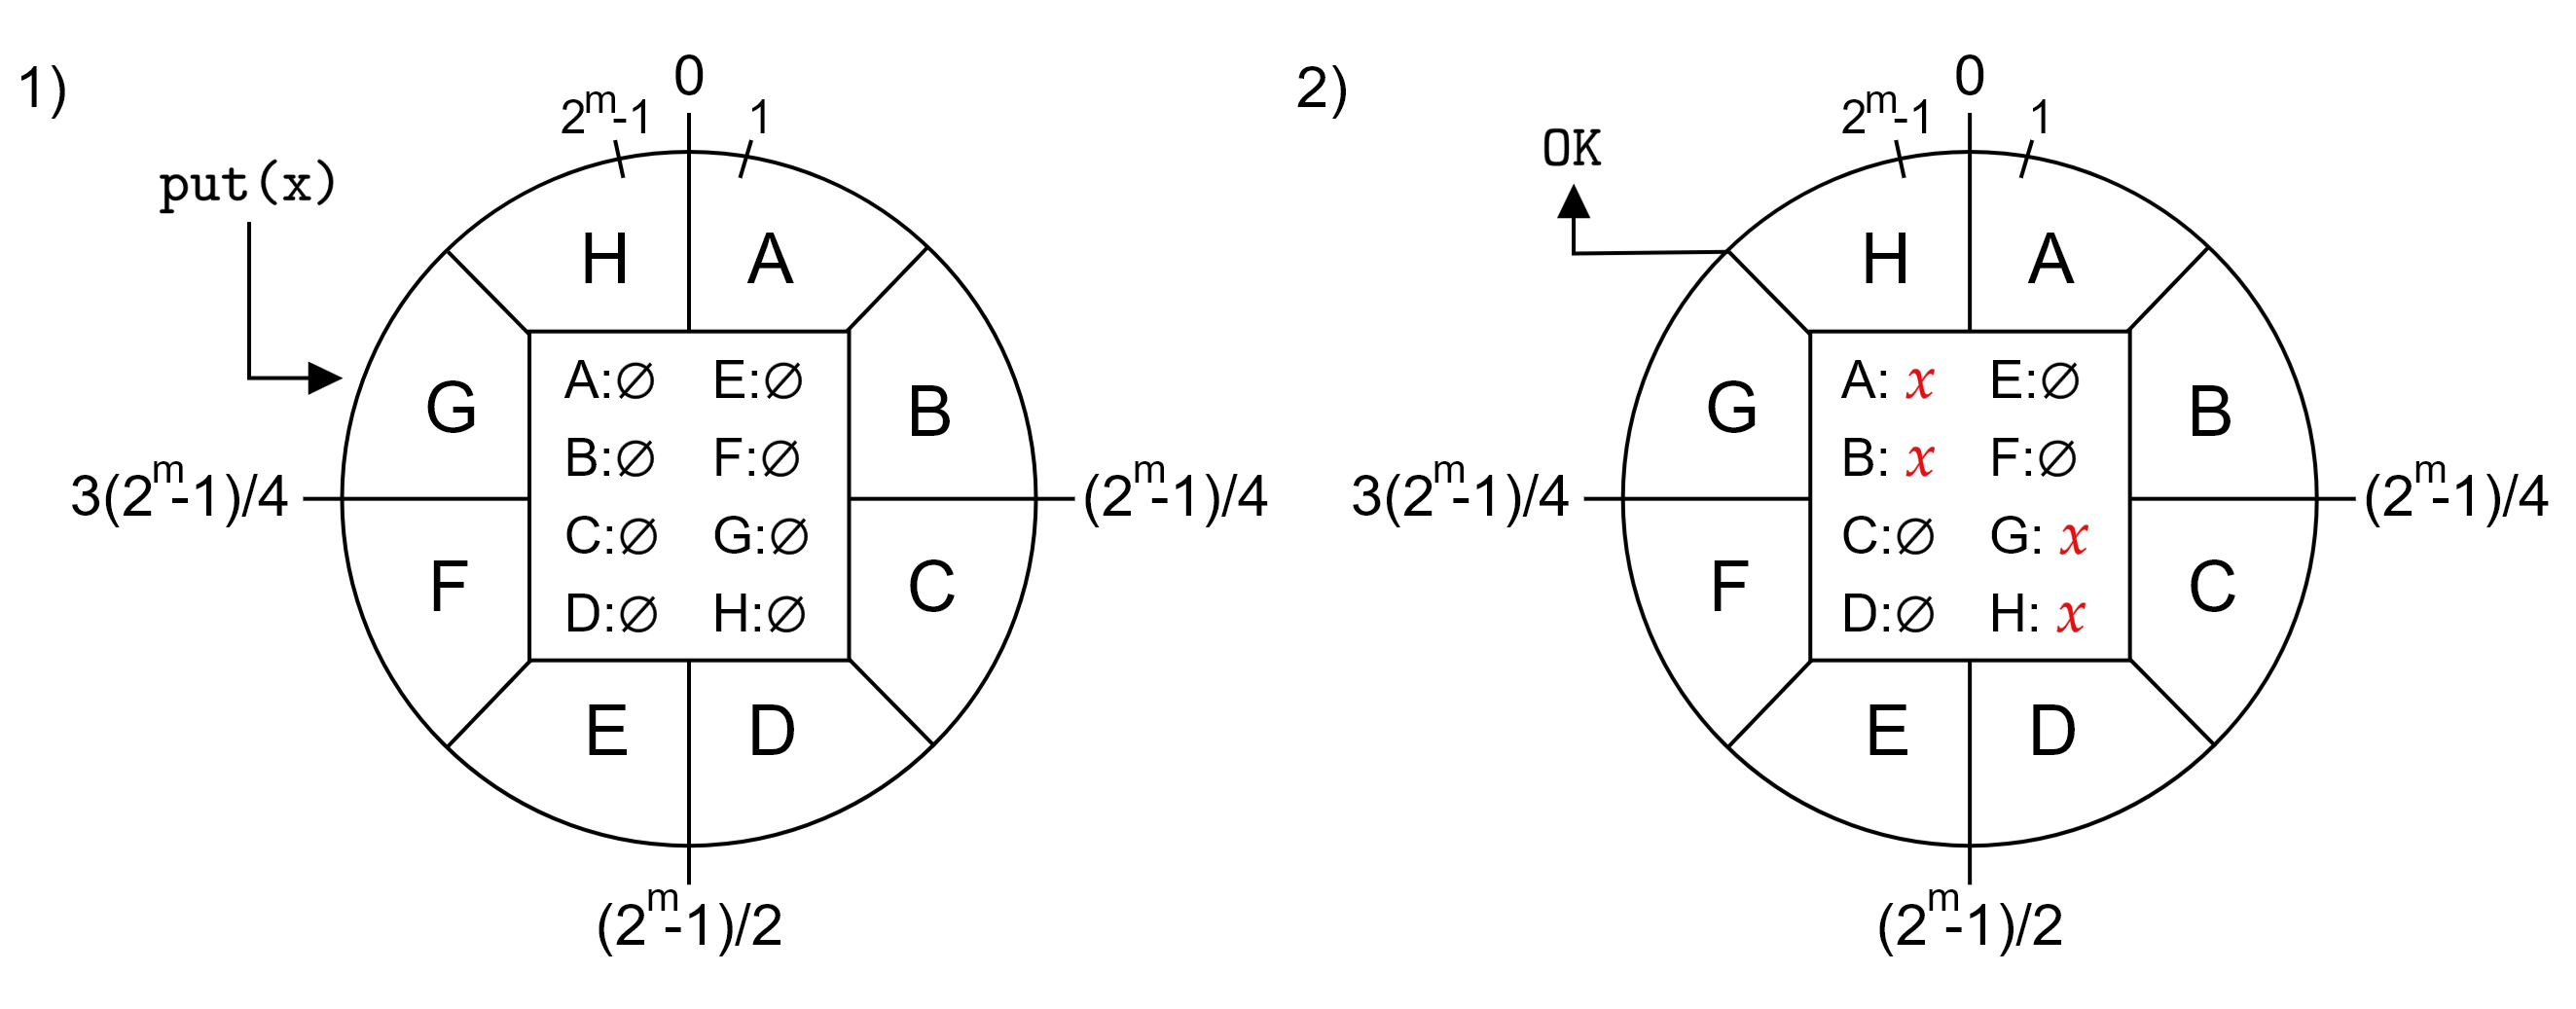
\includegraphics[width=\textwidth]{Sections/dyn/gossip.png}
        \caption{A basic quorum system. \textbf{To be clear}: virtual nodes are positioned at the spokes. For instance, \underline{$H$ starts at 0}, and ends at the next left-spoke $G$ (the top-left corner of the center box). Here, $R=4, W=4, N=7$, and servers are 
        an ordered list of virtual nodes $A$--$H$. Also, here we say \texttt{put(x)} for brevity, while it's actually \texttt{put(key,value)}.
        1) A client's put request falls within $G$'s range. 2) The next top $W-1$ nodes acknowledge, with $G$ sending back an \texttt{OK} (success).}
        \label{fig:quorum}
    \end{figure}

    \noindent
    Moving on, we deal with the liveness of nodes, and how to reconcile data:
    \begin{Def}[Quorum System -- Gossip \& Hints (Part 2)]

        Dynamo's monitors liveness with the following mechanisms:\\
      
        \noindent
        \textbf{Gossip Frequency \& Peer Selection:}  
        Every second, each node picks a random peer and exchanges its local membership-change log (join/leave/failure records). This gossip ensures that all nodes eventually learn who is up or down without any central service.\\
      
        \noindent
        \textbf{Failure Detection \& Sloppy Quorum:}  
        During a write, if a coordinator cannot reach a preferred replica (due to a failure or partition), it writes to the next healthy node in the preference list. That node stores the update alongside a \textbf{``hint''} tagging the intended replica.
        
        In particular, each node stores hints in a separate local database \underline{unbeknownst to the client}. This is called a \textbf{sloppy quorum}: it allows writes and reads to proceed even if some replicas are unreachable, as long as $W$ and $R$ are satisfied.\\
        
      
        \noindent
        \textbf{Hinted Handoff:}  
        When the failed node rejoins, any node holding a hint for it will detect its liveness via gossip and then forward the update it missed in a ``handoff''---restoring the full set of $N$ replicas \textbf{without} blocking client operations.
      \end{Def}

    \newpage 
    \noindent
    Below illustrates the gossip protocol and hinted handoff:
    \begin{figure}[h]
        
        \centering
        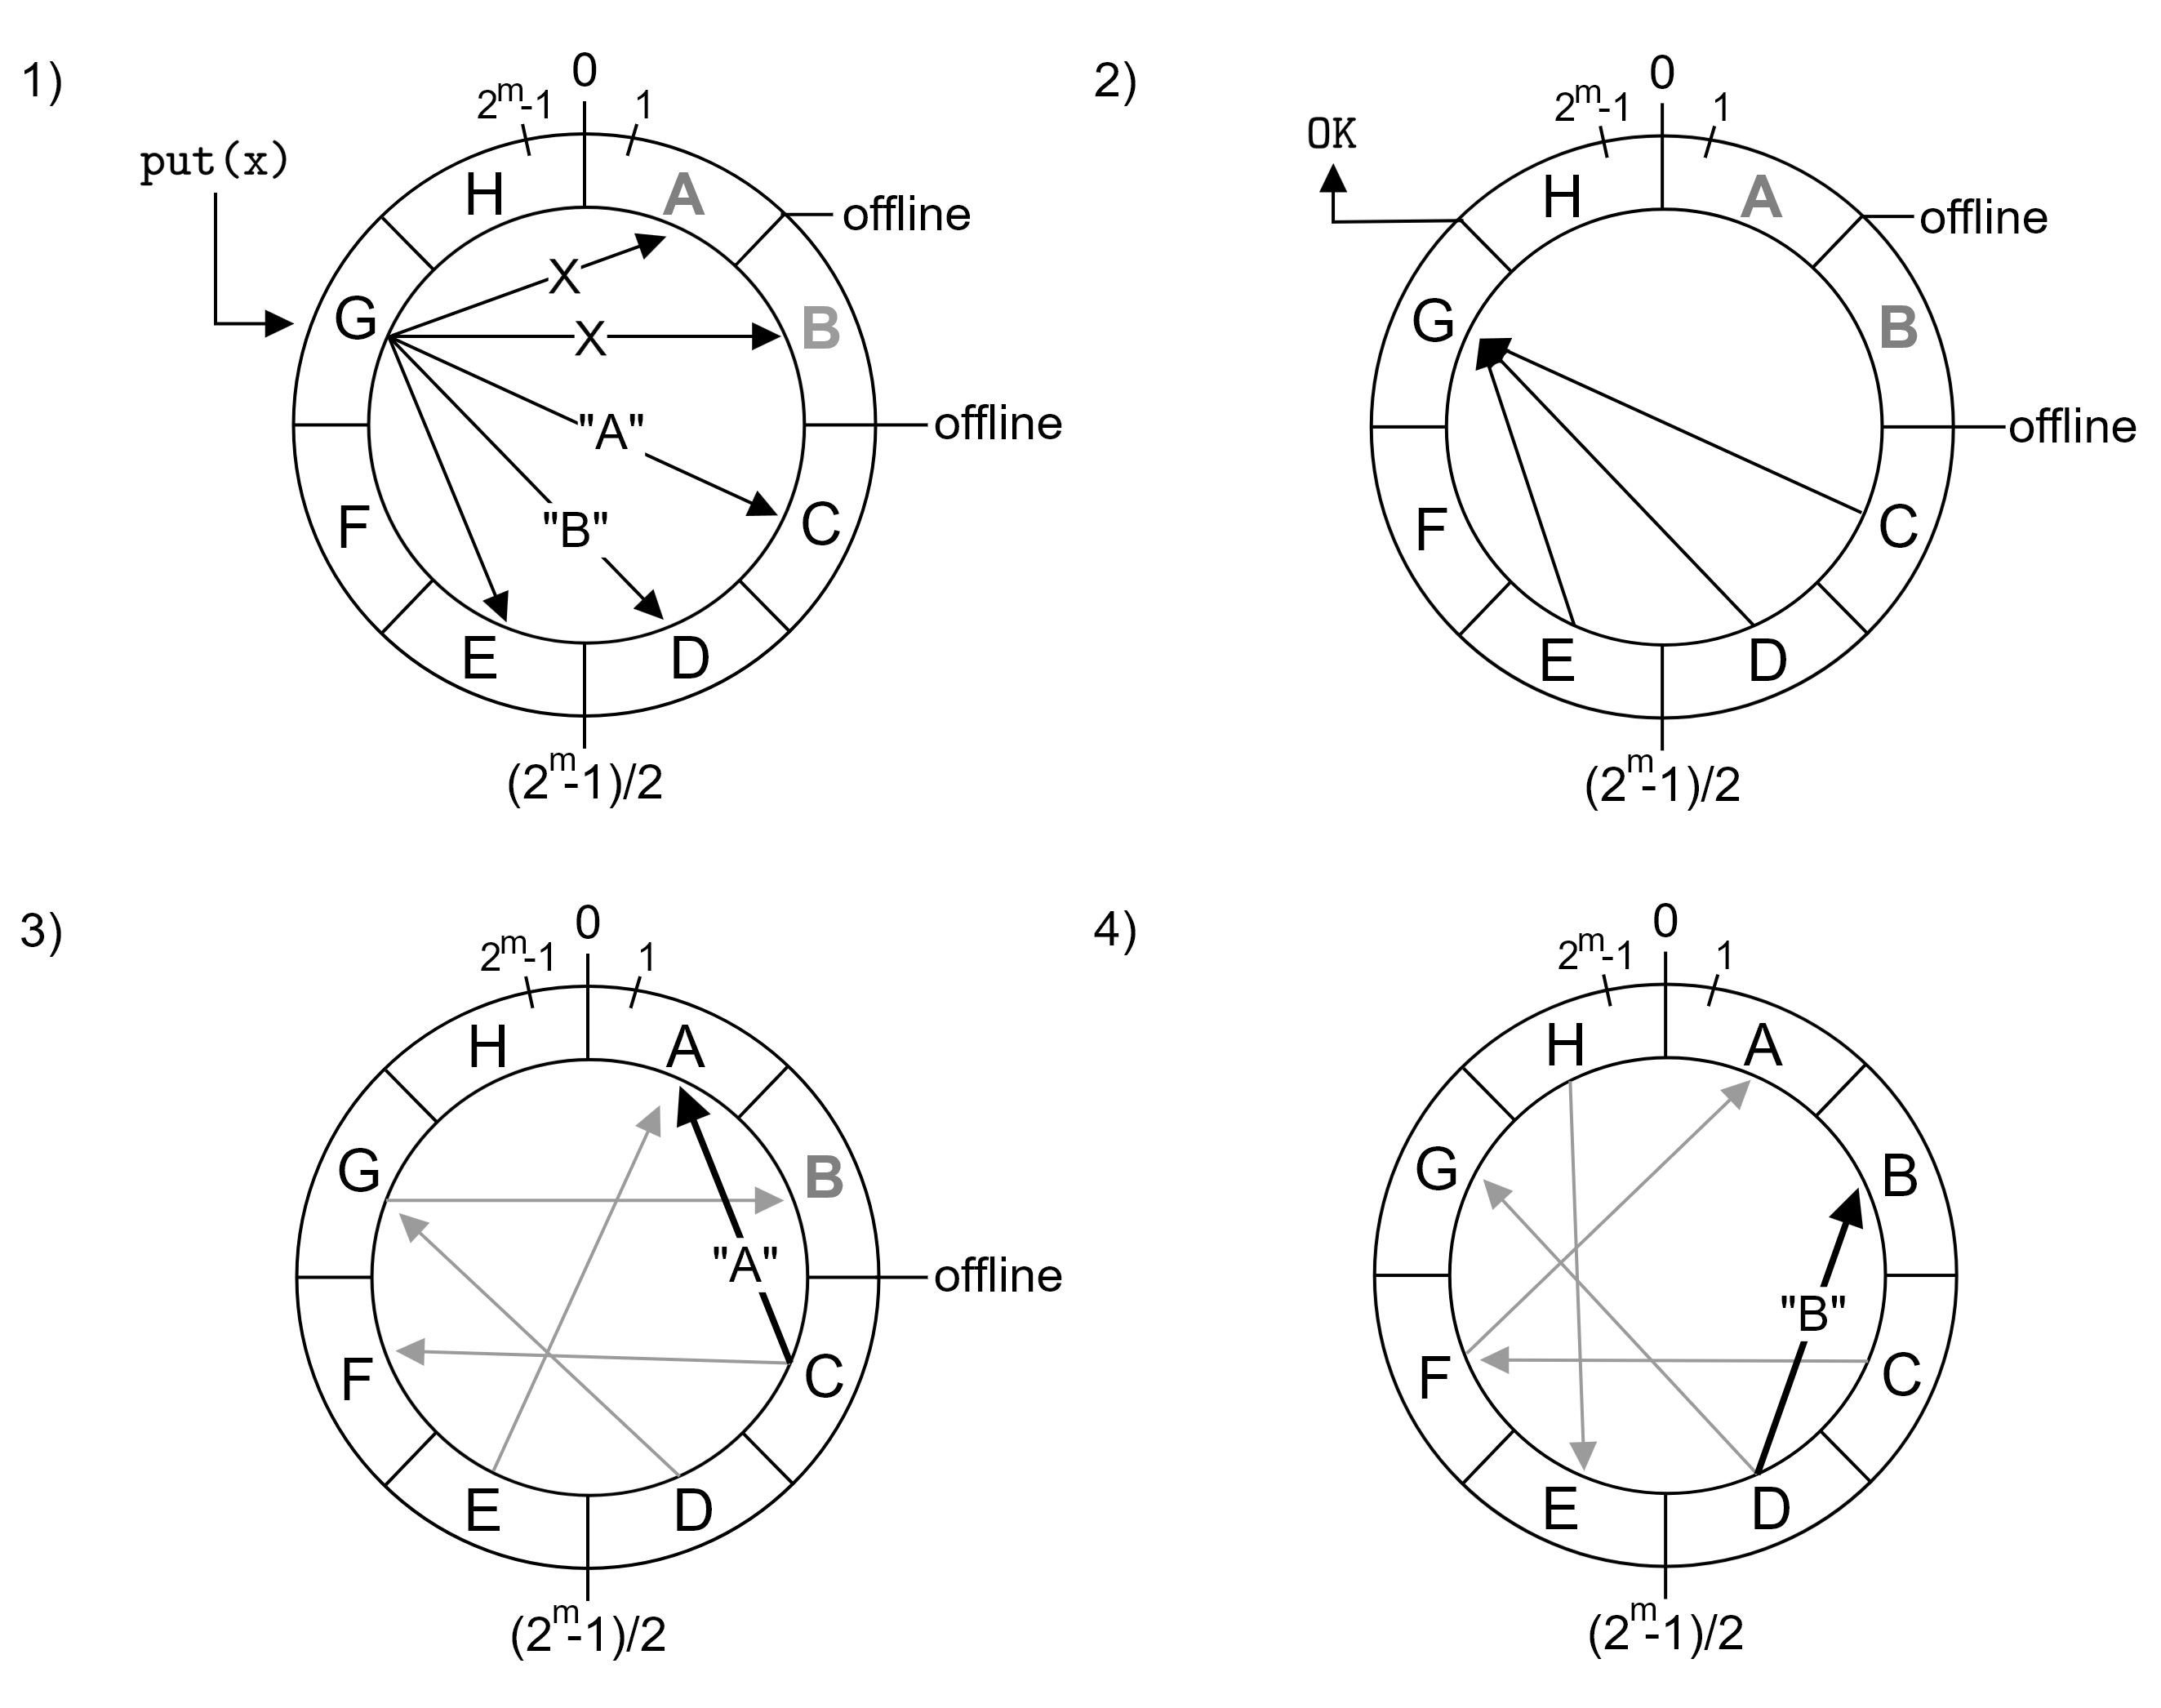
\includegraphics[width=\textwidth]{Sections/dyn/gossip_2.png}
        \caption{Gossip protocol and hinted handoff. 1) A put operation is sent to $G$, from which is then propagated. Though, $A$ and $B$ appear to be down, $G$ resolves this by giving hints to $C$ and $D$. 2) Nodes $C,D$ and $E$ \texttt{ACK}, allowing $G$ to return \texttt{OK}. 3) During the gossip protocol $A$ comes back online; $C$ notices this and sends the hint to $A$ (hinted-handoff). 4) Later in the 
        gossip protocol, $B$ comes back online; $D$ notices and hands off the hint to $B$. \underline{\textbf{Note}: The paper does not follow} the one-hint-per-replica assumption made in this figure. Also, $G$ \textbf{should actually} send the write in parallel to $H\to A\to B\to\dots$ (its first three successors), but for visual-clarity we began with $A$.}
        \label{fig:gossip}
    \end{figure}

    \vspace{-1em}
    \begin{Note}
        \textbf{Note}:
        The Dynamo paper doesn't bound hint capacity. Here we assume at most one hint per missing replica, which in the worst case could lose writes if that holder also fails. 
        We might instead store hints on the next $N$ healthy nodes, or allow multiple distinct hints per replica to improve safety.
        
        The paper does say, ``replicas will keep [hints] in a 
        separate local database that is scanned periodically.'' The use of the word \textbf{Database} suggests hints may be propagated generously.
    \end{Note}
    \newpage 

    \noindent
    Now we discuss in detail how dynamo utilizes \textbf{Vector Clocks} to reconcile divergent data:
    \begin{Def}[Quorum System -- Vector Clocks \& Reconciliation (Part 3)]

        Every object (key-value pair) in Dynamo is associated with a \textbf{vector clock} $VC$ that tracks the version history of the object. The $VC$ is composed of $N$ (node, counter) tuple pairs, maintaining a change history:
        
        \begin{itemize}
          \item \textbf{Stamping \& Propagation:}  
            A client invokes $\texttt{put}(k,v,VC_{\mathrm{ctx}})$ at the coordinator $N_i$, where $VC_{\mathrm{ctx}}$ is the $VC$ from the last read (\texttt{get()}). $N_i$ merges $VC_{\mathrm{ctx}}$, increments its own counter entry in $VC$, 
            stores $(k,v,VC)$ locally, and then sends the entire tuple $(k,v,VC)$ in parallel to the other $N-1$ replicas.
        
          \item \textbf{Primary Path:}  
            In the failure-free case, $N_i$ waits for $W$ acknowledgments (including itself) before replying success. Each replica simply stores the tuple under key $k$ in its local key-value store.
        
          \item \textbf{Failover Path:}  
            If $N_i$ is unreachable, the client retries $\texttt{put}(k,v,VC_{\mathrm{ctx}})$ at the next alive node in the preference list. That node becomes the temporary coordinator: 
            it fetches or merges existing clocks, stamps its own counter, performs a sloppy-quorum write of $(k,v,VC)$, and tags hints for any skipped replicas (including the primary).
        
          \item \textbf{Read Reconciliation:}  
            A client issues $\texttt{get}(k)$ to the coordinator, which polls all $N$ replicas and waits for the first $R$ responses $(v_j,VC_j)$. If one $VC_j$ strictly dominates the others, its $v_j$ is returned; if some $VC_j$ are concurrent, all corresponding $v_j$ are returned.
        
          \item \textbf{Application Merge:}  
            When multiple versions $(v_j,VC_j)$ arrive, it's up to the application to merge them (semantic reconciliation) into a single $v_{\mathrm{merged}}$ and $VC_{\mathrm{merged}}$, then issue a fresh $\texttt{put}(k,v_{\mathrm{merged}},VC_{\mathrm{merged}})$.
        \end{itemize}
        \end{Def}

        \begin{figure}[h]
            
                \centering
                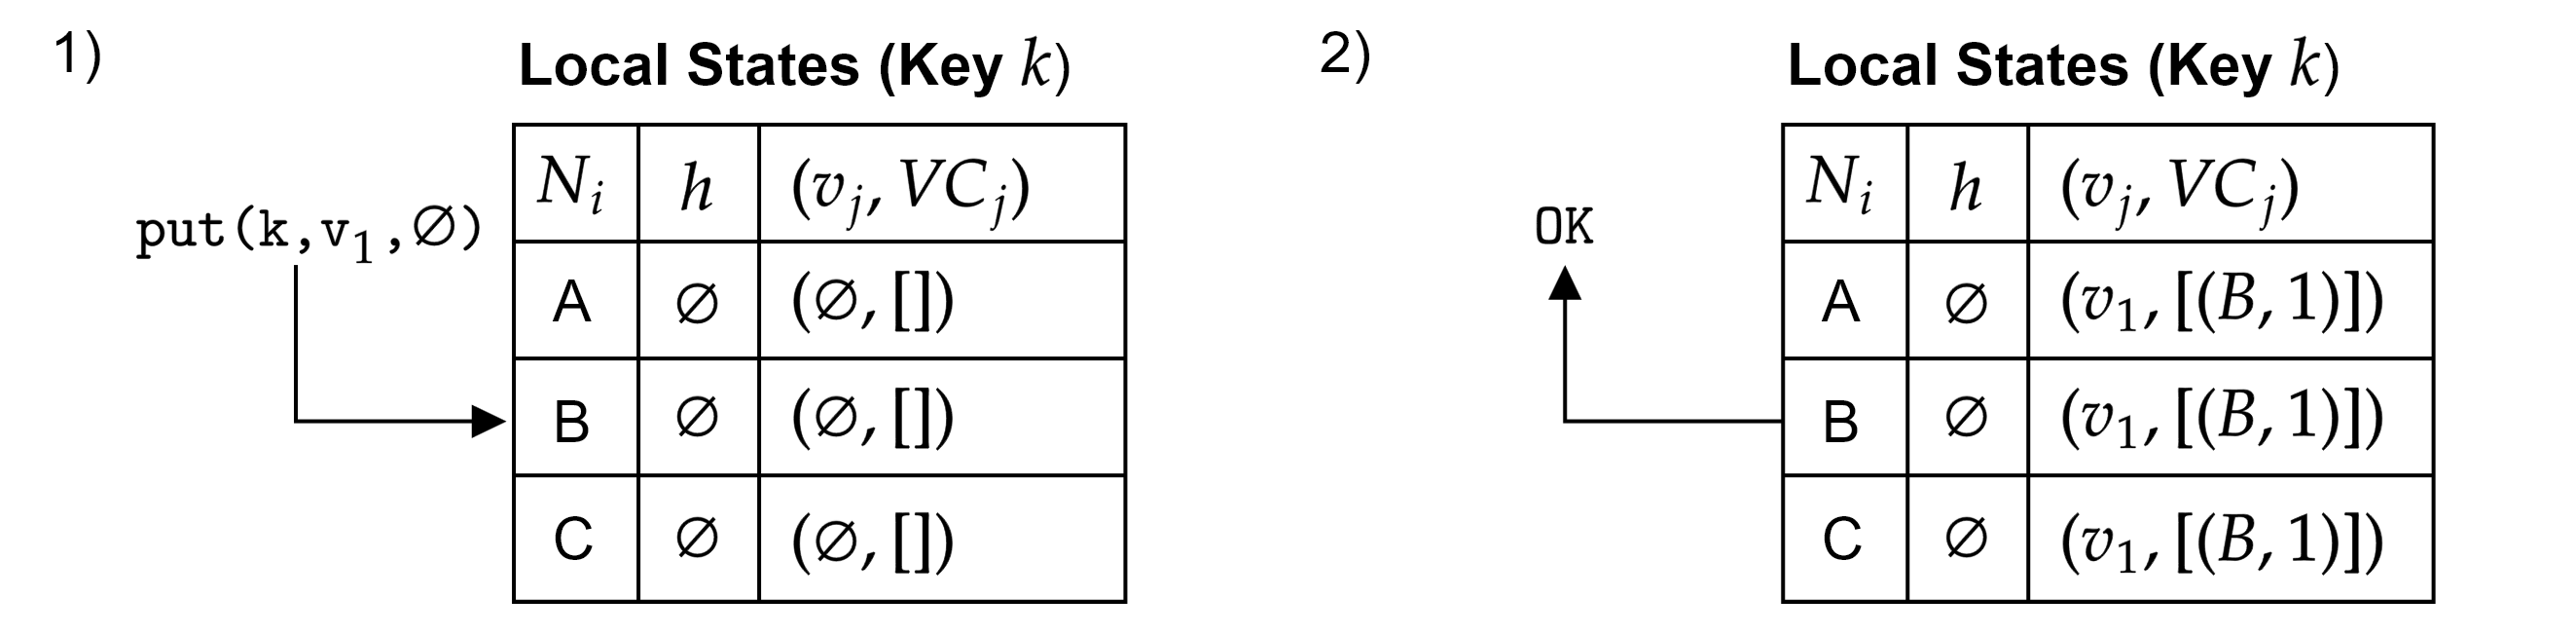
\includegraphics[width=\textwidth]{Sections/dyn/vc.png}
                \caption{A simplified view of a ring with three $N_i$ nodes, $A$, $B$, and $C$, $h$ hints, and a (value, vector clock) tuple $(v_j,VC_j)$. 1) A client issues their first put request of \texttt{put(k,v$_1$,$\varnothing$)} (empty context) to $B$. 2) $B$ stores the tuple, $(v_1, [(B,1)])$, 
                indicating the new value, and notes its participation in a vector clock $VC$. It propagates $(k,v_1,VC)$
                to $A$ and $C$, returning success to the client.}
                \label{fig:vc}
        \end{figure}
        
    
\newpage

\noindent
\begin{figure}[ht!]
    
        \centering
        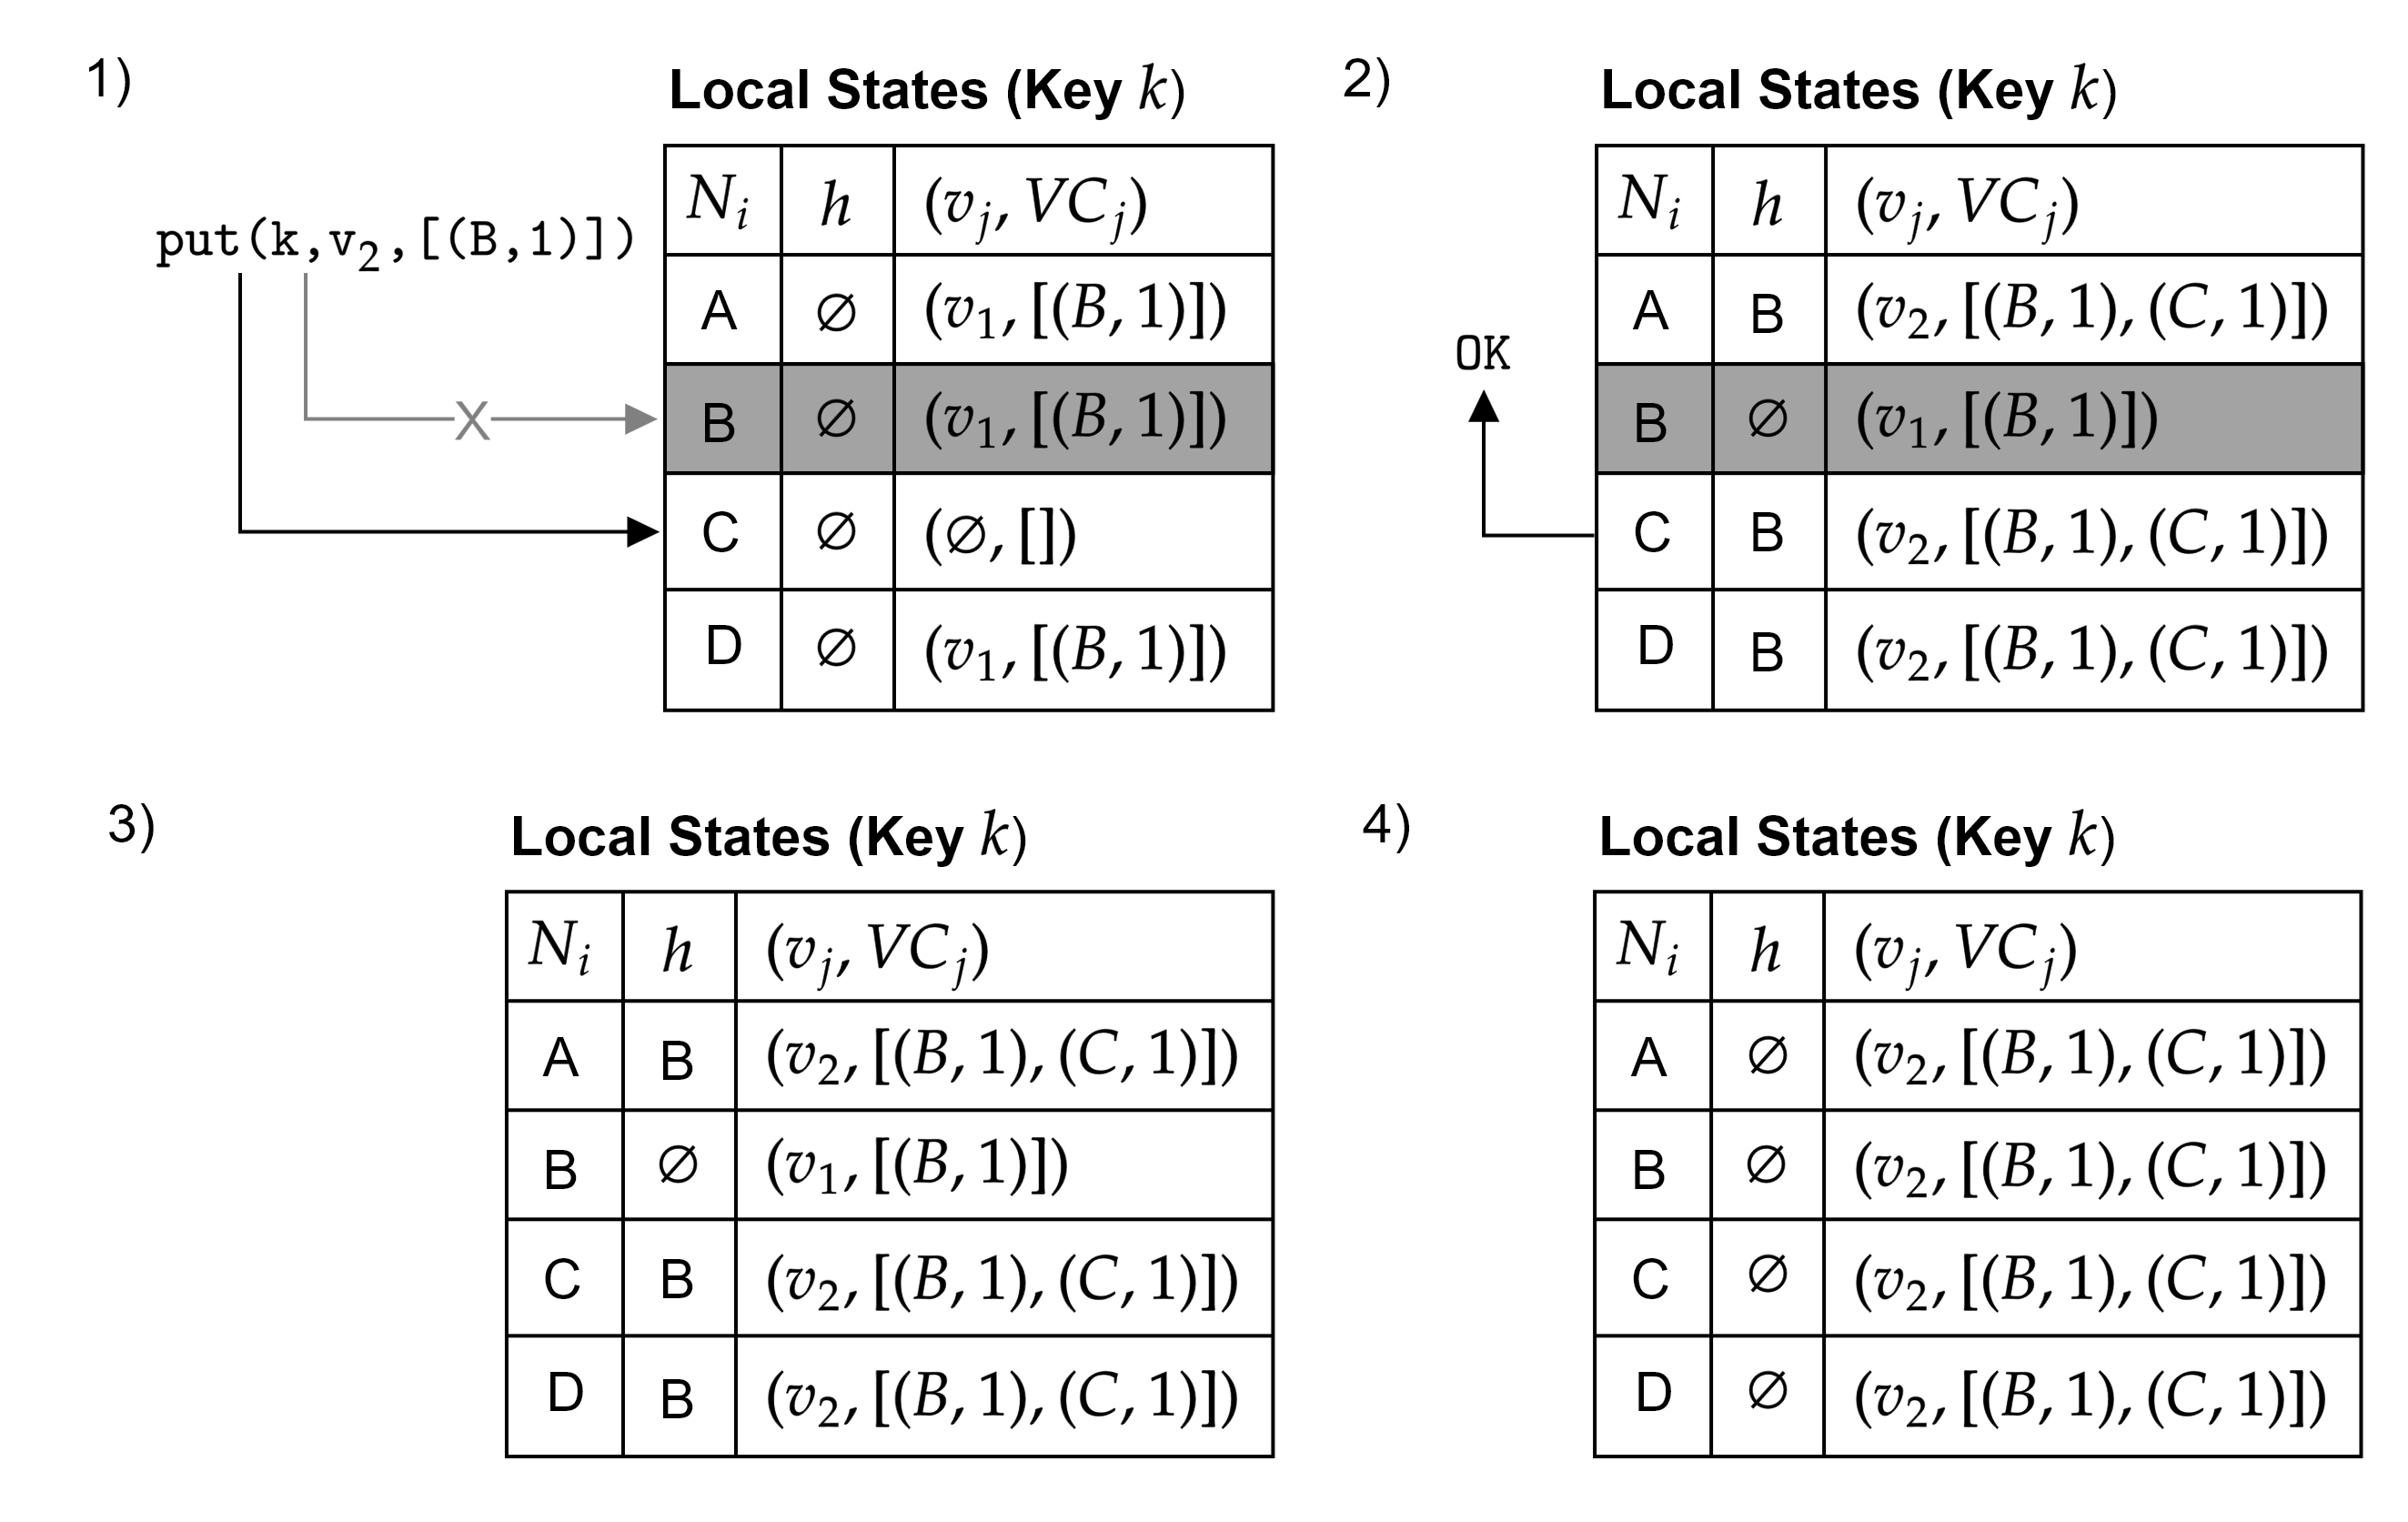
\includegraphics[width=.95\textwidth]{Sections/dyn/vc_2.png}
        \caption{ 1) A client issues a put request with \texttt{(k,v$_2$,[(B,1)])} implying a previous interaction of to $B$. Though, $B$ is down, and $C$ is the next alive node; However, $C$ has never seen $k$ before. $C$ takes the user's dominating input.
        2) $C$ stores the tuple, $(v_2, [(C,1),(B,1)])$, indicating the new value, and notes its participation in a vector clock $VC$. It propagates $(k,v_2,VC)$ with hint $B$ to $D$ and $A$, returning a success. 3) Later, $B$ rejoins during gossip. 4) A participants notice $B$'s revival, sending it updates.}
        \label{fig:vc_2}
\end{figure}

\vspace{-1em}
\begin{figure}[ht!]
        
            \centering
            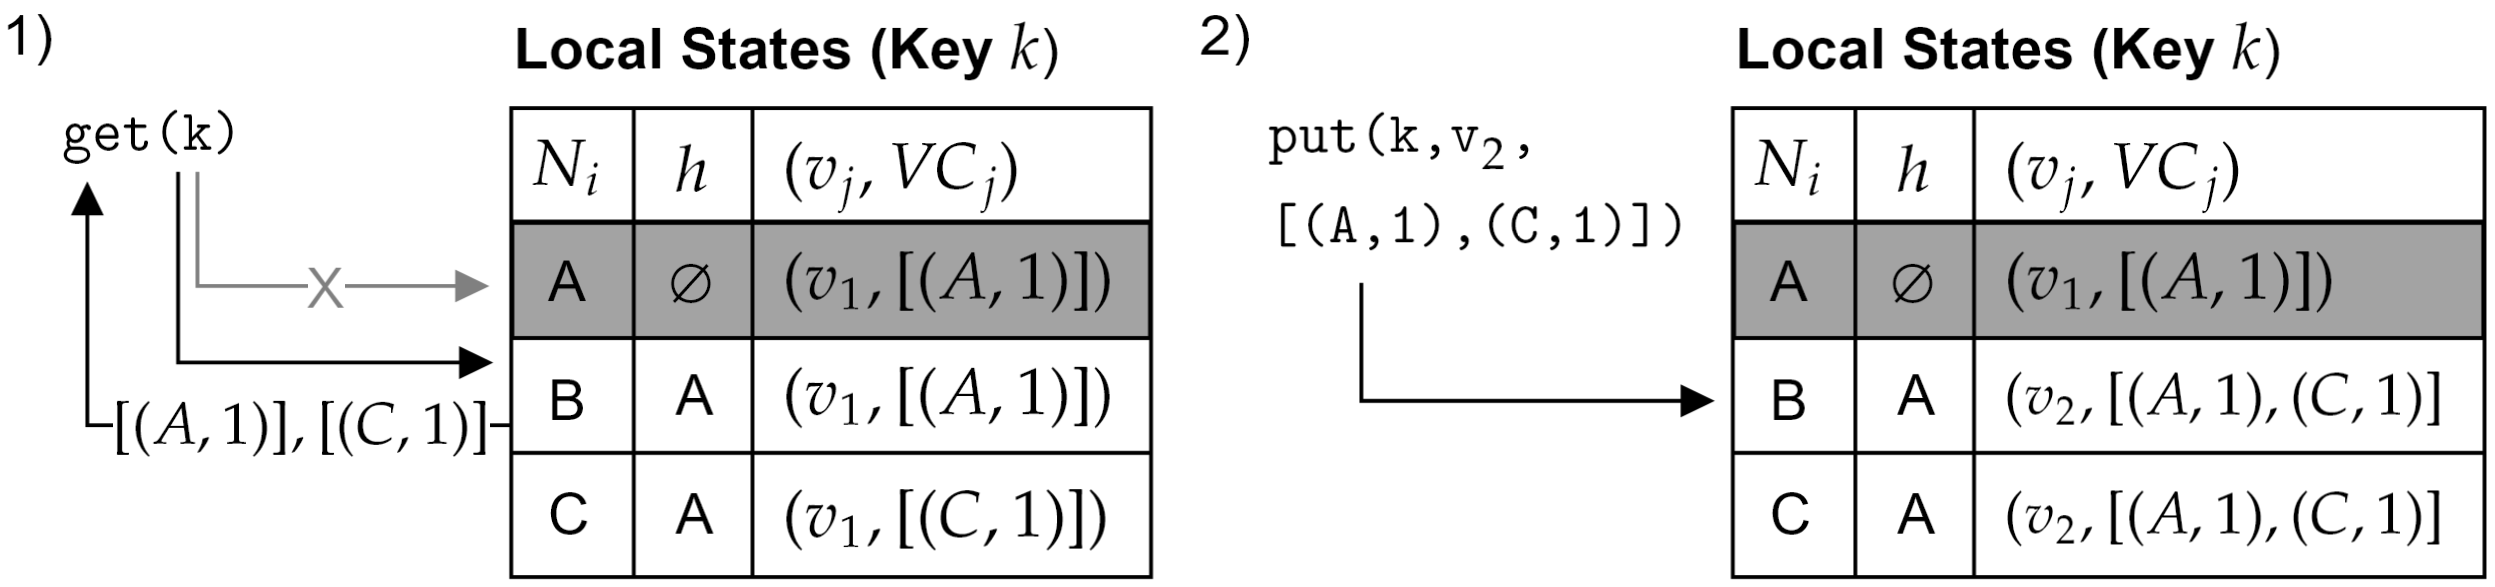
\includegraphics[width=.95\textwidth]{Sections/dyn/vc_3.png}
            \caption{ 1) The client requests key $k$ from $A$, but it's down, falling over to $B$, which gets a read from $C$;
            However, $C$'s entry is divergent, perhaps due to a network partition. To resolve, $B$ sends back both vectors, relying on the client to reconcile the data. 2) The client mends the data by merging the two vectors, pushing it 
            back to $B$. For example, a customer may have had two tabs open with different shopping carts. The application decides to merge the two carts, adding to the user experience.}
            \label{fig:vc_3}
\end{figure}

\newpage
\noindent
In an eventually-consistent store, vector clocks track the history of individual object updates but cannot tell us which keys out of millions have diverged across replicas. Dynamo employs the following technique to solve this problem efficiently:
\begin{Def}[Anti-Entropy via Merkle Trees]

    Dynamo uses Merkle trees to detect and repair divergent replicas without exhaustive scans:
    
    \begin{itemize}
      \item \textbf{Tree Construction:} Each node builds a binary Merkle tree over its local key-value store.  \textbf{Leaves} are the cryptographic hashes of individual key-value pairs (or small fixed-size batches of adjacent keys), computed as 
      \[
        H_i = \text{hash}(k_i \Vert v_i)\,
      \]
      .Then each \textbf{internal node} hashes the concatenation of its two children,
      where ($\Vert$) denotes concatenation, and $H$ is a cryptographic hash function (e.g., SHA-1, MD5). The root hash summarizes the entire tree.
      \item \textbf{Root Comparison:} Replicas exchange only their root hashes.  A match means the entire key-value set is identical—no further work.
      \item \textbf{Recursive Descent:} On a root mismatch, only the child hashes of the differing subtrees are exchanged, descending the tree until the exact leaf hashes (and thus specific keys) that differ are isolated.
      \item \textbf{Selective Synchronization:} Once out-of-sync keys are pinpointed, only those individual $(k,v)$ pairs (and their vector-clock metadata) are transferred and reconciled.
      \item \textbf{Efficiency Gains:} By limiting data exchange to mismatched branches, this method drastically reduces both network bandwidth and disk I/O compared to full scans.
    \end{itemize}
    \end{Def}
    
\begin{figure}[h]
            
            \centering
            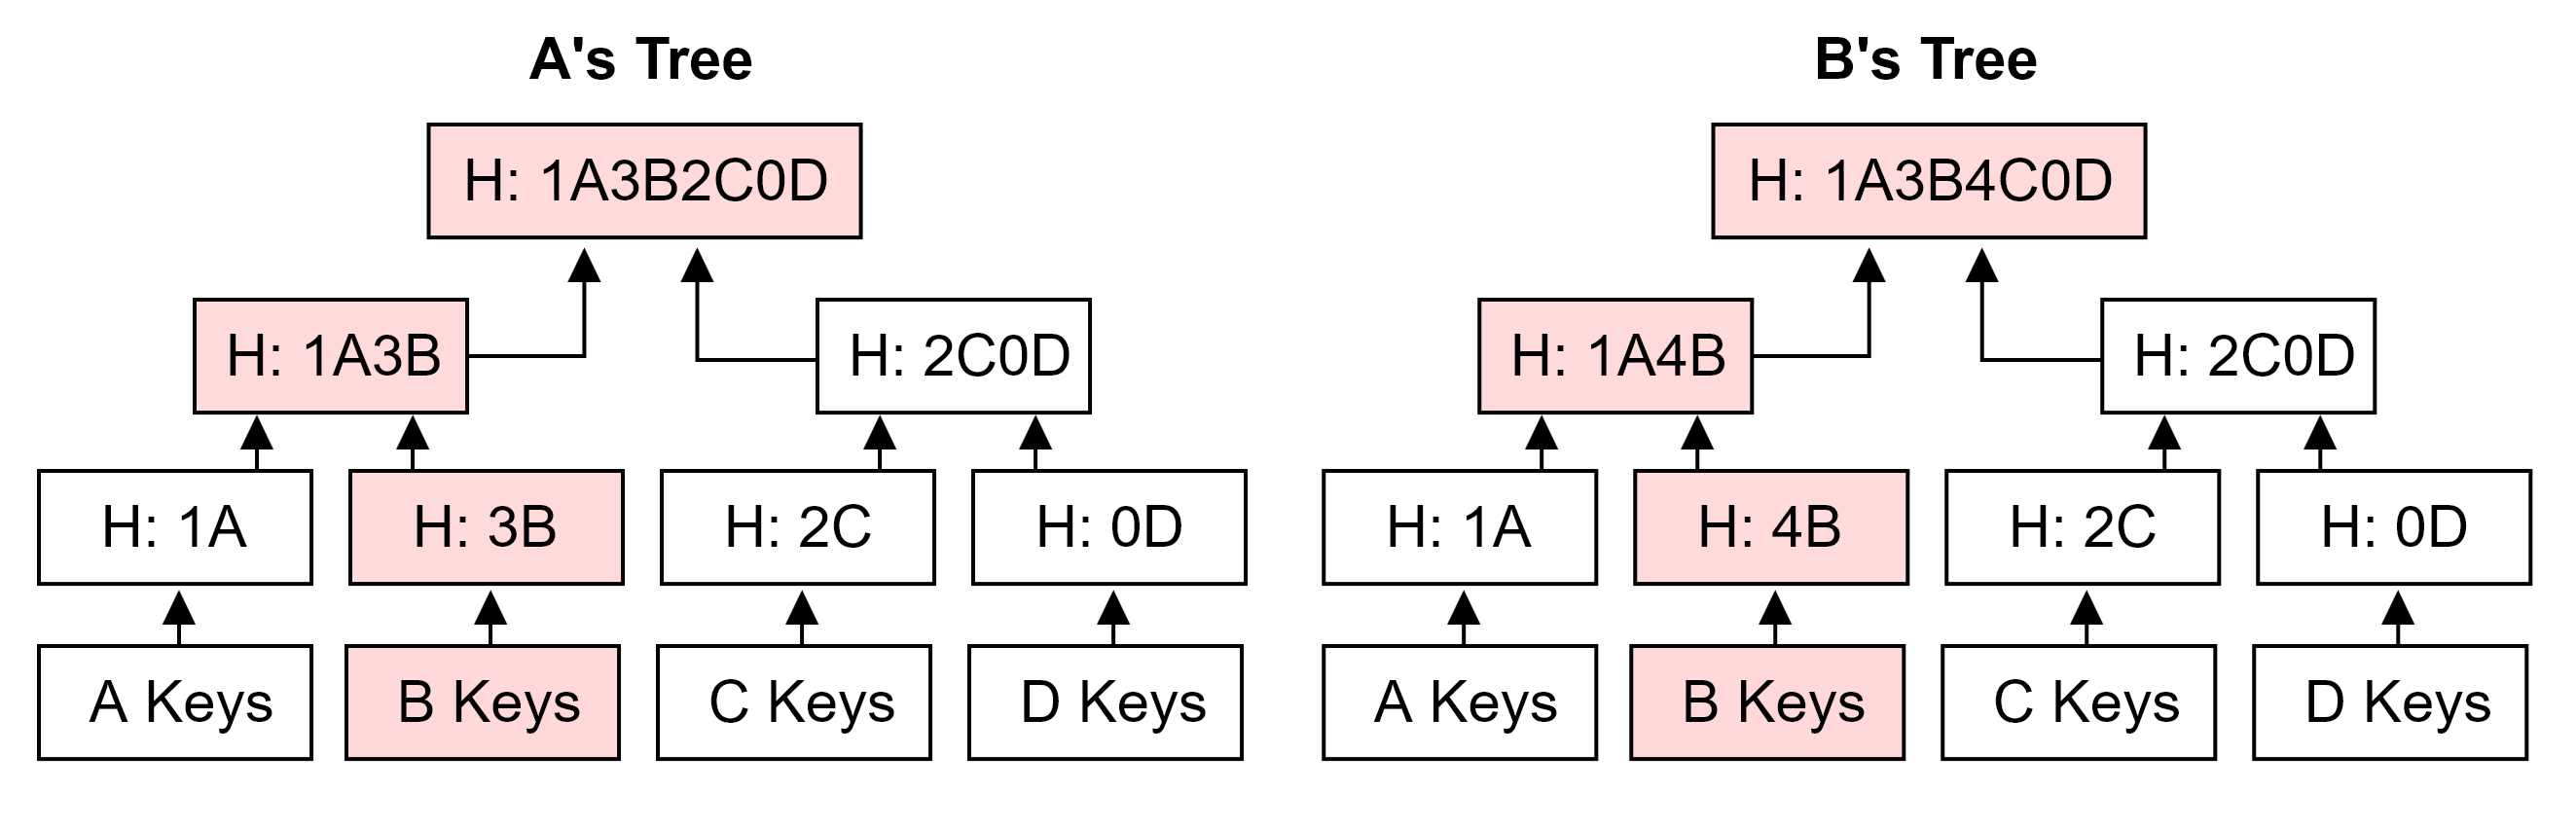
\includegraphics[width=.95\textwidth]{Sections/dyn/merkle.png}
            \caption{Given some arbitrary simplified hashing function, we construct a Merkle tree over key ranges $A$--$D$. Here $A$ and $B$ compare root hashes. They differ, so they descend to the branch 
            which causes the mismatch. They both discover a discrepancy in their $B$ key ranges.}
            \label{fig:merkle}
\end{figure}
